\documentclass[paper,oneside,onecolumn,notitlepage,bibtotocnumbered,fontsize=12pt,bigheadings,ngerman]{scrartcl}
\usepackage[singlespacing]{setspace}
\usepackage[ngerman]{babel}
\usepackage{fancyhdr}                          
\pagestyle{fancy} 
\usepackage[parfill]{parskip}                        
\addto\captionsngerman{
\renewcommand{\figurename}{Abbildung}
\renewcommand{\tablename}{Tab.}
}
\newcommand{\thema}{CAD-Project - Mom based Information Live Flow}
\newcommand{\schlagworte}{MoM, IoT, Cloud, CEP}
\newcommand{\zusammenfassung}{
}

\newcommand{\autor}{Paul Drautzburg,  Lukas Hansen,  Georg Mohr, Kim De Souza, Sebastian Thuemmel, Sascha Drobig}

%Encodingeinstellung
\usepackage[utf8]{inputenc}
%Packete zur Formatierung von Tabellen und Grafiken
\usepackage{graphicx}
\usepackage{tabularx}
\usepackage{multicol}
\usepackage{float}
\usepackage{floatflt}
\usepackage{here}
\usepackage{blindtext}
\usepackage{wrapfig}
\usepackage{bigstrut}
\usepackage{subfloat}
\usepackage{subfigure}
%\usepackage{scrpage2} 
%\pagestyle{scrheadings}
\usepackage[small]{titlesec}
\usepackage{colortbl}	
\usepackage{cite}
\usepackage{hyperref}
\usepackage{amsmath}
\usepackage{nicefrac}
\usepackage{pstricks}
\usepackage{pst-3dplot}
\usepackage{glossaries}
\usepackage{listings}
\usepackage{needspace}
\usepackage[nottoc]{tocbibind}
%\pagestyle{myheadings}
%\clearscrheadfoot
\renewcommand{\thefootnote}{\arabic{footnote}} 


%Titelseite (optional)
\newcommand{\sectionnumbering}[1]{% 
  \setcounter{section}{0}% 
   \renewcommand{\thesection}{\csname #1\endcsname{section}}} 
   
   
   
\usepackage{caption}
\DeclareCaptionFont{white}{\color{white}}
\DeclareCaptionFormat{listing}{\colorbox{gray}{\parbox{\textwidth}{#1#2#3}}}
\captionsetup[lstlisting]{format=listing,labelfont=white,textfont=white}




\usepackage{listings}


\begin{document}
\shorthandoff{"}
\pagenumbering{roman} 
\include{cover}

\include{title}

{\Large \textbf{Vorwort}}
\bigskip

Das vorliegende Dokument beschreibt grob eine Idee und das Vorgehen für die Umsetzung für das Projekt im Rahmen der Master Veranstaltung \textit{Cloud Application Development}.
\include{affidavit}
\include{abstract}


\normalsize


\setlength{\parindent}{0pt}

\newpage
\sectionnumbering{Roman} 
\tableofcontents
\clearpage

\listoffigures 
\clearpage 

\listoftables 
\clearpage
\pagenumbering{arabic} 
\sectionnumbering{arabic} 

\section{Problemstellung}
Wir erhalten eine große Menge an Sensordaten die zur Verarbeitung und Erfassung von Wetterdaten, Berechnung von Statistiken und Erstellung von Wetterwarnungen verwendet werden sollen. Der Eingang der Wetterdaten erfolgt kontinuierlich und Belastungsspitzen sind nur in Ausnahmefällen zu erwarten. Zusätzlich sollen beliebige zusätzliche Wetterdaten in den Verarbeitungsprozess integriert werden können. 
Da zum Empfang der Daten und anschließenden Verarbeitung kein Server vollständig ausgelastet wird, soll das System in einer Cloud-Lösung ausgelagert werden. 
Des Weiteren ist die Cloudlösung nötig, da wir keine eigene Server-Infrastruktur betreiben wollen oder können, da dies aus finanzieller, organisatorischer und infrastruktureller Sicht vorteilhaft ist.

\section{Lösungsansatz}
In diesem Abschnitt wird vorerst auf eine kurze Beschreibung für die im vorhergehenden Kapitel beschriebenen Problemstellung eingegangen. Anschließend wird aus  der allgemeinen Beschreibung eine erste Anforderungsdefinition an eine Softwarelösung abgeleitet.
\subsection{Allgemein}
Der Ansatz einer angemessenen Softwarelösung schließt drei heterogene Systeme mit ein. 

Diese drei heterogenen Systeme bestehen aus
\begin{itemize}
\item Sender von Wetterdaten,
\item Anwendung für \textit{Complex Event Processing},
\item Clients zum Empfang und zum Darstellen der aufbereiteten Wetterdaten und Warnungen,
\end{itemize}
sollen durch eine \textit{Message-oriented Middleware} (MoM) kommunizieren. Die MoM soll im allgemeinen Sensordaten verarbeiten können, welche 
aus prinzipiell jeder Art von Binärdaten bestehen können, somit kann diese MoM gleichzeitig für andere Szenarien verwendet werden. 

Im vorliegendem Fall beschränken sich die zu verarbeitenden Daten auf Wetterdaten aus einer Wetter-API. Diese angesprochenen Wetterdaten können sowohl als Json wie auch als XML abgezogen werden. Um die Auslastung einer Instanz steuern zu können, wird die MoM auch fingierte Wetterdaten weiterleiten können und durch Complex Event Processing (CEP) verarbeiten können. Ein weiterer Hintergrund für diese Entscheidung war die Richtigkeit der errechneten Daten. Die Wetterdaten der API können, zu keinem Zeitpunkt, genau vorhergesagt werden und somit können die Ergebnisse des CEP nicht auf Richtigkeit validiert werden. 

Ferner soll die Lösung bei einer vorher definierten Systemauslastung weitere Ressourcen dazuschalten können. 

Die Abbildung 1. zeigt das Ergebnis eines Brainstormings, welches als Grundlage für einen Lösungsansatz dient.

\begin{figure}[!ht]
\centering
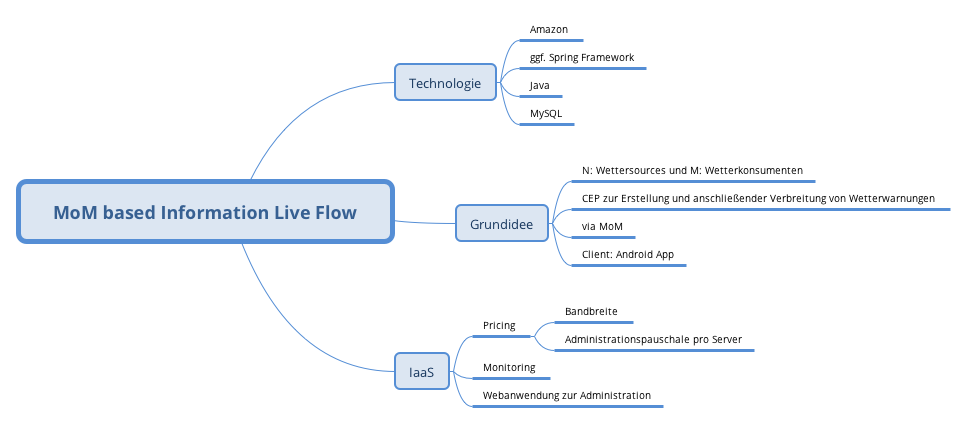
\includegraphics[width=450pt]{MoM based Information Live Flow.png}
\caption{Brainstorming}
\end{figure}

Die folgende Abbildung 2. zeigt die grobe System-Architektur. Die wichtigsten Bestandteile dieser sind:
\begin{itemize}
\item Sensoren (Dateninput)
\item MoM
\item CEP
\item Database
\item Android-Client
\item Web-Client
\end{itemize}
\begin{figure}[!ht]
\centering
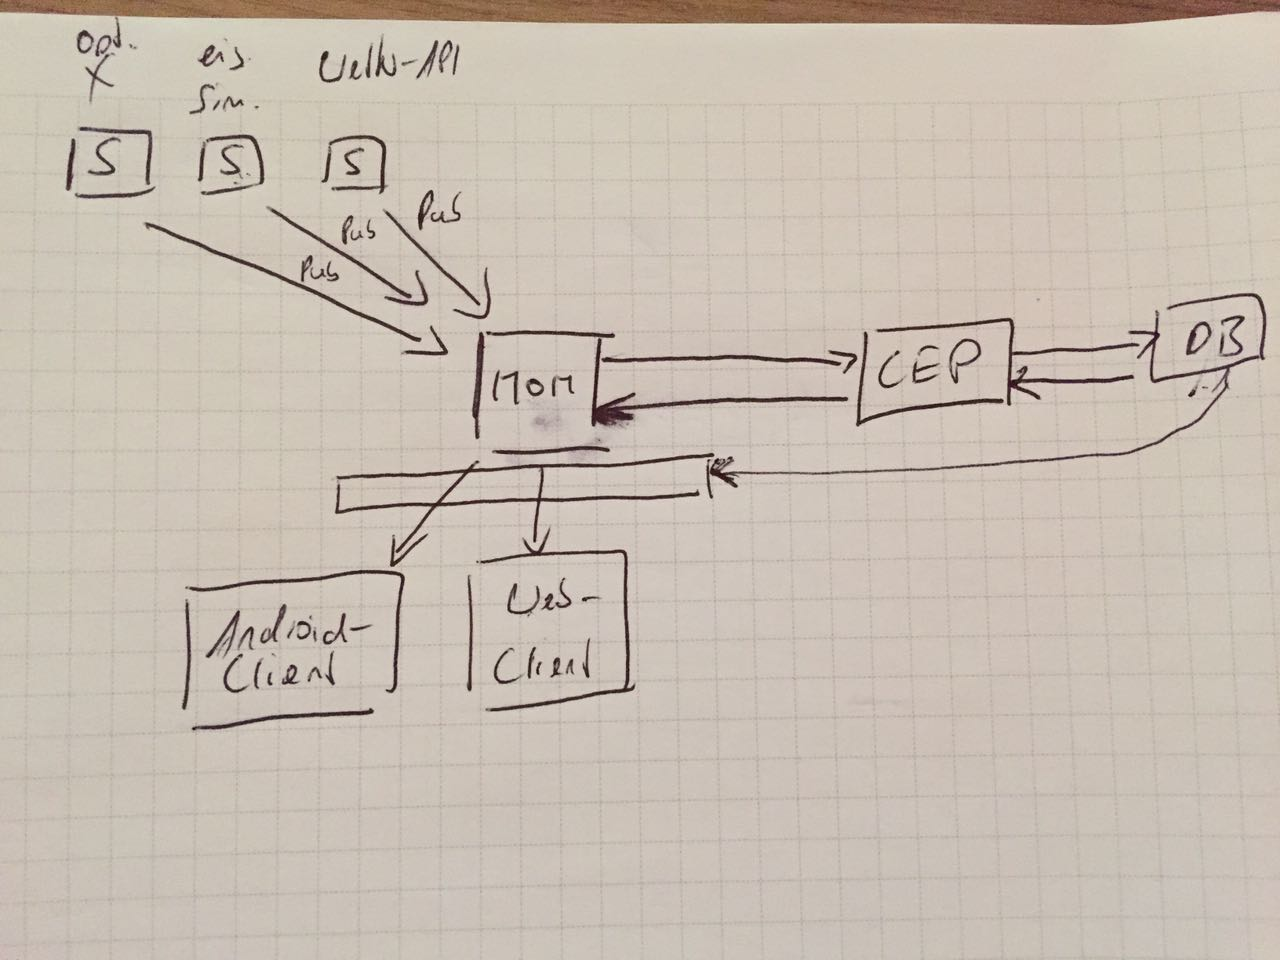
\includegraphics[width=450pt]{System-Archtitektur.jpeg}
\caption{Grobe System-Architektur}
\end{figure}
\clearpage

\subsection{Anforderungsdefiniton}
Aus dem im letzten Abschnitt allgemein Beschriebenen können folgende grundlegenden nicht-funktionalen und funktionalen Anforderungen an ein System abgeleitet werden. 

Die folgende Tabelle beschreibt die Kernanforderungen jeweils getrennt in nicht-funktionale und funktionale Anforderungen,
\begin{table}[!ht]
  \centering
    \begin{minipage}{15cm}
      \centering
      \begin{tabular}{*{3}{|l|p{5.0cm}|p{5.0cm}}}\hline
     ID&Anforderung&Beschreibung\\\hline
  
\multicolumn{3}{|c|}{\cellcolor[RGB]{200,200,200}Nicht-funktionale Anforderungen} \\\hline
    
     1.1&Multi-tenancy&Das System muss eine fehlerfreie Mehrnutzer Funktionalität erfüllen\\
      \hline
     1.2&Scalability&Das System muss in der Lage sein zu jeder Zeit skalieren zu können\\
     \hline
     1.3&Fault-tolerance&Das System muss auf Fehler von Nutzer in angemessenem Rahmen reagieren\\
     \hline
     1.4&Cloudarchitektur&Das System muss vollständig in einer Cloudbasierten Umgebung lauffähig sein\\
     \hline
\multicolumn{3}{|c|}{\cellcolor[RGB]{200,200,200}Funktionale Anforderungen} \\\hline   
 
     1.4&Binäre Daten annehmen&Das System soll binäre Daten annehmen können\\
     \hline
     1.5&Daten aufbereiten& Die Daten werden nach einem Muster aufbereitet\\
     \hline
      1.6& Daten abonnieren&Die Daten können von Abonnenten bezogen werden.\\
     \hline
      1.7&Nutzerverwaltung&Die User sollen in einer Datenbank verwaltet werden können.\\
     \hline
       1.9&Statistikfunktion&Die gespeicherten Daten sollen mit Hilfe einer Statistikfunktion aufbereitet werden können.\\
     \hline
     1.9&Datenquelle&Die Daten sollen via Wetter App bezogen werden können\\
\hline     
     2&Datenquelle&Die Daten sollen mit einem Generator fingiert werden können\\
\hline
2.1&Complex Event Processing&Aus den analysierten Daten sollen mit Hilfe von CEP verschiedene Ereignisse ausgelöst werden können.\\
     \hline
      \end{tabular}
   \caption{Funktionale Anforderungen an den Prototyp}\label{tab:Anforderungen1}
    \end{minipage}
\end{table}
\clearpage


\section{Testing}

Im letzten Abschnitt dieser Projektbeschreibung wird auf das Testing eingegangen. Hierbei wird zwischen den Kernpunkten Skalierbarkeit und Ausfallsicherheit/Multi-Tendency unterschieden, auf diese wird in den folgenden Abschnitten eingegangen.

\subsection{Skalierbarkeit}
\begin{itemize}
\item Normallast:	definierter Input durch Wetterdaten API mit bestimmter Clientzahl für Performancebalancing 
Bestimmung von Grenzwerten (Scalingparameter) für Optimale Systemsicherheit (Datenkonsistenz/Datentransferraten etc.)
\item Client - Stresstest:	definierte Menge an Topics werden  zur Verfügung gestellt. Schrittweise wird die Anzahl der Clientanschlüsse (virtuell) erhöht.  
Mithilfe der Scalingparameter (Normallast) muss das Cloud System weitere Ressourcen in Anspruch nehmen und der Output muss bewältigt werden(Datensicherheit\- /Zugriffsteuerungen/etc.) können. Der Latenzvergleich mit optimaler Normallast ergibt das Maß für Skalierbarkeit des Systems.
\item Inputdaten - Stresstest:	eine definierte Anzahl an Clients verbindet sich mit dem System und bezieht Daten aus der MoM. Mit Hilfe einer eigenen Softwarelösung werden nun fingierte Wetterdatenmengen in das System (MOM) eingespeist.
\begin{itemize}
\item Skalierungsparameter (Normallast) Input muss bewältigt werden
\item Latenzvergleich  (Datentransfer von Input bis Output auf einem Client) mit Optimaler Normallast ergibt Maß für Skalierbarkeit des Systems
\end{itemize}
\item Abnahmetest: Test und finale Analyse des gesamten Cloudsystems 
Verschiedene Szenarien  (Normallast, Client-Veränderungen, InputDaten-Veränderungen) werden in verschiedenen Kombinationen und Ausprägungen in das System gespeist.
\item Finale Testinganalyse (Gesamtsystem)
\item Modulparameter Fine-tuning der AWS Cloud Architecture
\clearpage
\end{itemize}

\subsection{Ausfallsicherheit/Multi-Tendency}

\begin{itemize}

\item MoM- Clients:	Topics von anderem User dürfen nicht zur Verfügung gestellt werden. Zeitlich simultane Abfrage gleicher oder minimal abweichender Topics.		
\begin{itemize}
\item Test des Zugriffsverfahrens IAM (Amazon Web Services Identity and Access Management) Hinweis: Analog zu Keystone Identity Modul (OpenStack)
\end{itemize}


\item CEP - Datenbank:Datenkonsistenz bei Lastverhalten
(siehe Szenarien der der Skalierbarkeit)
\begin{itemize}
\item Prüfung der Ergebnisse (Topics)
\item Prüfung über Statistikvergleiche möglich (Rahmen für zu erwartenden Wert versus geliefert/berechneter Wert) 
\end{itemize}



\item Clients - Datenbank:	User hat die Möglichkeit ein Userprofil anzulegen (Suchkriterien zu speichern/Statistiken anzusehen)
\begin{itemize}
\item Test des Userzugriffs Datensicherheit (Test der Oracle Userrollenzugriffe bzw. Test der Einstellungen im Modul IAM)
\end{itemize}
\end{itemize}

\end{document}
